Most of the muons produced in CMS originate in processes such as semileptonic decays of top quarks or heavy-flavor hadrons, or in leptonic decays of on-shell vector bosons ($Z$, $W$).
Such muons typically have $p_{T} < 200 GeV$, and are referred to as low-$p_{T}$ muons.
On the other hand, high-$p_{T}$ muons are produced in rare processes like from the decay of hypothetical beyond the standard model (BSM) particles such as $Z'$ or $W'$ bosons with TeV-scale mass.

Experimentally, the main differences between high- and low-$p_{T}$ muons can be understood as follows.
As the muon momentum increases, the $p_{T}$ resolution of the reconstructed track degrades. In the part of the orbit in near-uniform magnetic field $B$, the measurement of $p_{T}$ depends on $B$, and the radius of curvature, $R$, of the track:

\begin{equation}
  p_{T}[\text{GeV}] = \left|0.3 B[\text{T}] R[\text{m}]\right|.
\label{eq:pTvsRadius}
\end{equation}
The magnetic field is monitored with high precision and is roughly uniform at 3.8 T in the tracker volume inside the solenoid. The radius of curvature is related to the arc length $L$ and sagitta $s$, defined in Figure \ref{fig:SagittaDef},  of the track via

\begin{equation}
  R[\text{m}]\approx L[\text{m}]^{2}/8s[\text{m}],
\label{eq:RadiusvsSagitta}
\end{equation}
where the approximation is valid for $L/R \ll 1$. Assigning arithmetic signs consistently to $R$, $s$, and the charge $q$ (in units of proton charge) yields
\begin{equation}
  s[\text{m}]\approx (0.3 B [\text{T}] L[\text{m}]^{2}/8) (q/p_{T}[\text{GeV}]) =  (0.3 BL^{2}/8) \times (q/p_{T}),
\label{eq:SagittavsPt}
\end{equation}

\begin{figure}
\centering
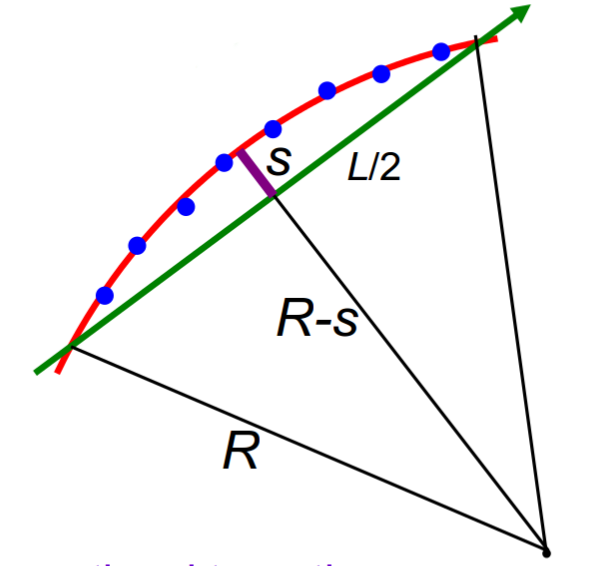
\includegraphics[width=0.30\textwidth]{figures/curvaturesketch.png}
\caption{Definition of saggita, $s$, from the length of of the reconstructed track, $L$, and its radious, $R$.}
\label{fig:SagittaDef}
\end{figure}

Inspecting Equations \eqref{eq:pTvsRadius} and \eqref{eq:RadiusvsSagitta} one can make two observations. Firstly, sagitta is proportional to the inverse of the transverse momentum, $s\sim1/p_{T}$. As a consquence, the muon curvature, $\kappa=q/p_{T}$, provides a direct probe of the experimental observable sagitta and is often used in the note for muon resolution/scale studies. Secondly, as the $p_{T}$ increases for a fixed value of $L$, sagitta decreases. In order to improve the resolution at small sagitta, the global muon track reconstruction relies on the matching of tracks reconstructed in different subdetectors (tracker and muon system) separated more than 3 meters away and effectively leads to tracks with a larger values of sagitta by using larger reconstructed tracks. The inclusion of hits in the muon system leads to sizable improvements in the muon $p_{T}$ resolution. This solution is used by default for the muon $p_{T}$ measurement when $p_{T}>200$~GeV. Lastly, due to the smallness of sagitta at the TeV regime, the muon $p_{T}$ resolution is sensitive to mismeasurements of sagitta caused by a non-perfect alignment of the hits used to reconstruct the muon track. Misaligments can affect tracks recontructed in the inner tracker alone or in the combination of inner tracker with muon system information.

On the other hand, when muons travelling in iron have sufficiently large momentum,  $p_{T} > {\cal O}(200~$GeV), the radiative energy losses (ee pair production, bremsstrahlung and photonuclear interactions) are not negligible compared to ionization energy losses.  Figure~\ref{fig:dEdX} shows the energy loss per unit of distance, $dE/dx$, for muons travelling through hydrogen, iron and uranium as a function of its energy.

\begin{figure}
\centering
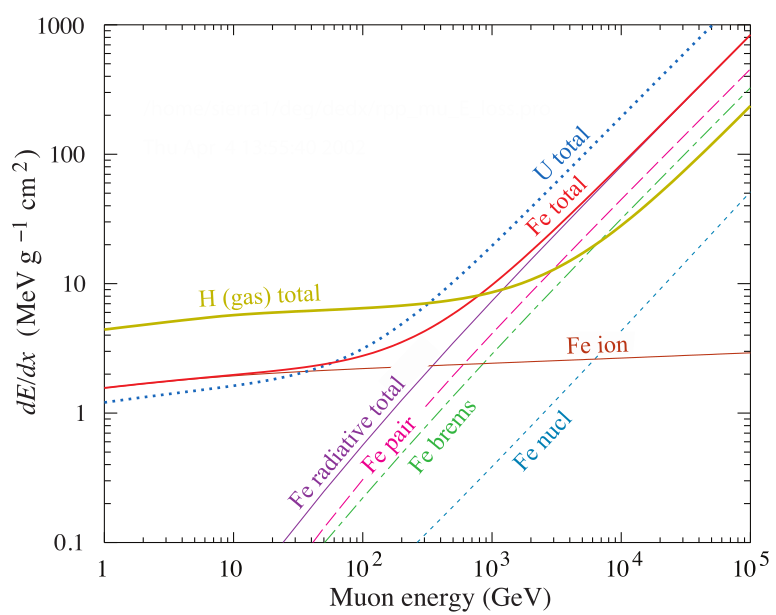
\includegraphics[width=0.60\textwidth]{figures/dEdx.png}
\caption{Average energy loss from ionization and radiative loss of a muon in hydrogen, iron and uranium as a function of its energy. Separate contributions to $dE/dx$ in iron from ee pair production, bremsstrahlung and photonuclear interactionsfor are also shown. Figure from \cite{Tanabashi:2018oca}.}
\label{fig:dEdX}        
\end{figure}


In the same Figure, contributions in iron from ionization (brown), ee pair production (pink), bremstrahlung (green) and photonuclear interactions (blue) are shown separately.  The muon critical energy for iron, $E^{iron}_{c}$, where the ionization energy losses (brown) are equal to the sum of all radiative losses (purple) occurs around 300 GeV. As a consequence, the main source of energy losses for muons with $E>E^{iron}_{c}$ travelling in the iron between the different muon subdetectors is due to electromagnetic (EM) radiation (electrons and photons). This EM radiation is called muon shower and can lead to extra hits and segments in the muon detectors that affect the muon performance (i.e triggering, reconstruction or $p_{T}$ measurement). Since the muon showering primarly depends on the muon energy and not the transverse momentum, it is often studied in the note as a function of $p$ instead of $p_{T}$.


Taking a simulated $Z'$ sample, the momemtum resolution can be measured as: 

\begin{equation}
\ensuremath{R_{\mathrm{reco}\textrm{-}\mathrm{gen}}} =
\frac{(q/p)^{\mathrm{reco}} - (q/p)^{\mathrm{gen}}}{(q/p)^{\mathrm{gen}}}
\label{resolution}
\end{equation}

where $q/p$ corresponds to the muon charge divided by its momentum.
